\section{Introduction}

Drivers enter a parking lot without having any specific knowledge about the
lot's availability. Especially in urban areas, it is common for any driver to
spend an additional, non-trivial amount of time looking for a parking spot. This
searching time not only translates into frustration but also wastes energy and
produces carbon dioxide harmful for the environment.

In order to assist drivers searching for a parking space, numerous smartphone
applications are developed and available in the online application stores such
as Google Play Store and App Store. Although many drivers find these smartphone
applications useful, these applications either do not provide real-time parking
lot availability or just display publicly-accessible availability information.

To overcome this limitation, a few academic systems have been
proposed~\cite{4212497, Chen:2012:COS, Delot:2009:CRP, 5062057,
Mathur:2010:PDS}. However, these systems make various assumptions that prevent
them from being immediately deployable. Typical assumptions include the
availability of additional infrastructure~\cite{5062057}, additional equipment
deployed on vehicles~\cite{Mathur:2010:PDS}, the presence of a vehicular
network~\cite{Delot:2009:CRP, Mathur:2010:PDS, 4212497}, and manual inputs from
users~\cite{Chen:2012:COS}.

We present {\it PocketParker}, a system that predicts parking lot availability
using smartphones. Unlike previous approaches, our goal is to not require any
additional input or infrastructure other than the smartphones used by the users
of PocketParker. More specifically, we only require our users to download a
smartphone application that runs in the background and detects parking related
events. Using this information, we construct a prediction model that estimates
the availability of a parking lot in our backend server. This simple operational
requirement gives PocketParker the advantage of being easily deployable. In
general, we consider our approach to be an example of a special type of
crowdsourcing that does not require any manual user input. We term {\it
pocketsourcing} to refer to this type of crowdsourcing.

Our goal of pocketsourcing accompanies two technical challenges. The first
challenge is detecting parking related events accurately while minimizing energy
consumption; the second challenge is accurately predicting parking lot
availability in the presence of {\it hidden drivers} who do not use our
smartphone application. We address the first challenge by designing a simple,
yet effective event detector; our event detector mainly relies on the
accelerometer on a smartphone to detect park and depark events, which is more
energy-efficient than GPS. We address the second challenge by designing an
availability estimator that probabilistically predicts the availability of a
parking lot based on the events reported by our event detector; our prediction
model estimates arrival and departure rates for a parking lot and adjusts the
availability probability accordingly.

To validate the effectiveness of PocketParker, we evaluate each of our
techniques in a setting best suited for assessing the technique. We evaluate
our parking event detector in a controlled environment with eight volunteers
participating in ten parking scenarios. We design a simulator to evaluate our
parking availability estimator, which gives us the flexibility to experiment
with a variety of parameters and parking lot types. Finally, we evaluate the
overall effectiveness of PocketParker by deploying it with five smartphones used
by our participants over ten days. To obtain ground truth, we deploy four
cameras that monitor four parking lots over two weeks. We inspect and hand-code
one day's worth of images for two parking lots to measure their true
availability. Altogether, our results show the efficiency and accuracy of
PocketParker.

The rest of our paper is organized as follows. We start by presenting related
work in Section~\ref{sec-related} in order to distinguish PocketParker from
multiple previous efforts at parking monitoring. Next, in
Sections~\ref{sec-detector}~and~\ref{sec-model} we describe the two major
components of PocketParker: our parking event detector and availability
model. Our evalution in Section~\ref{sec-evaluation} uses several approaches
to evaluate PocketParker, including controlled experiments, simulations, and
a small deployment. Finally, we discuss limitations and future work in
Section~\ref{sec-future} before concluding in Section~\ref{sec-conclusions}.

\begin{figure}
\centering
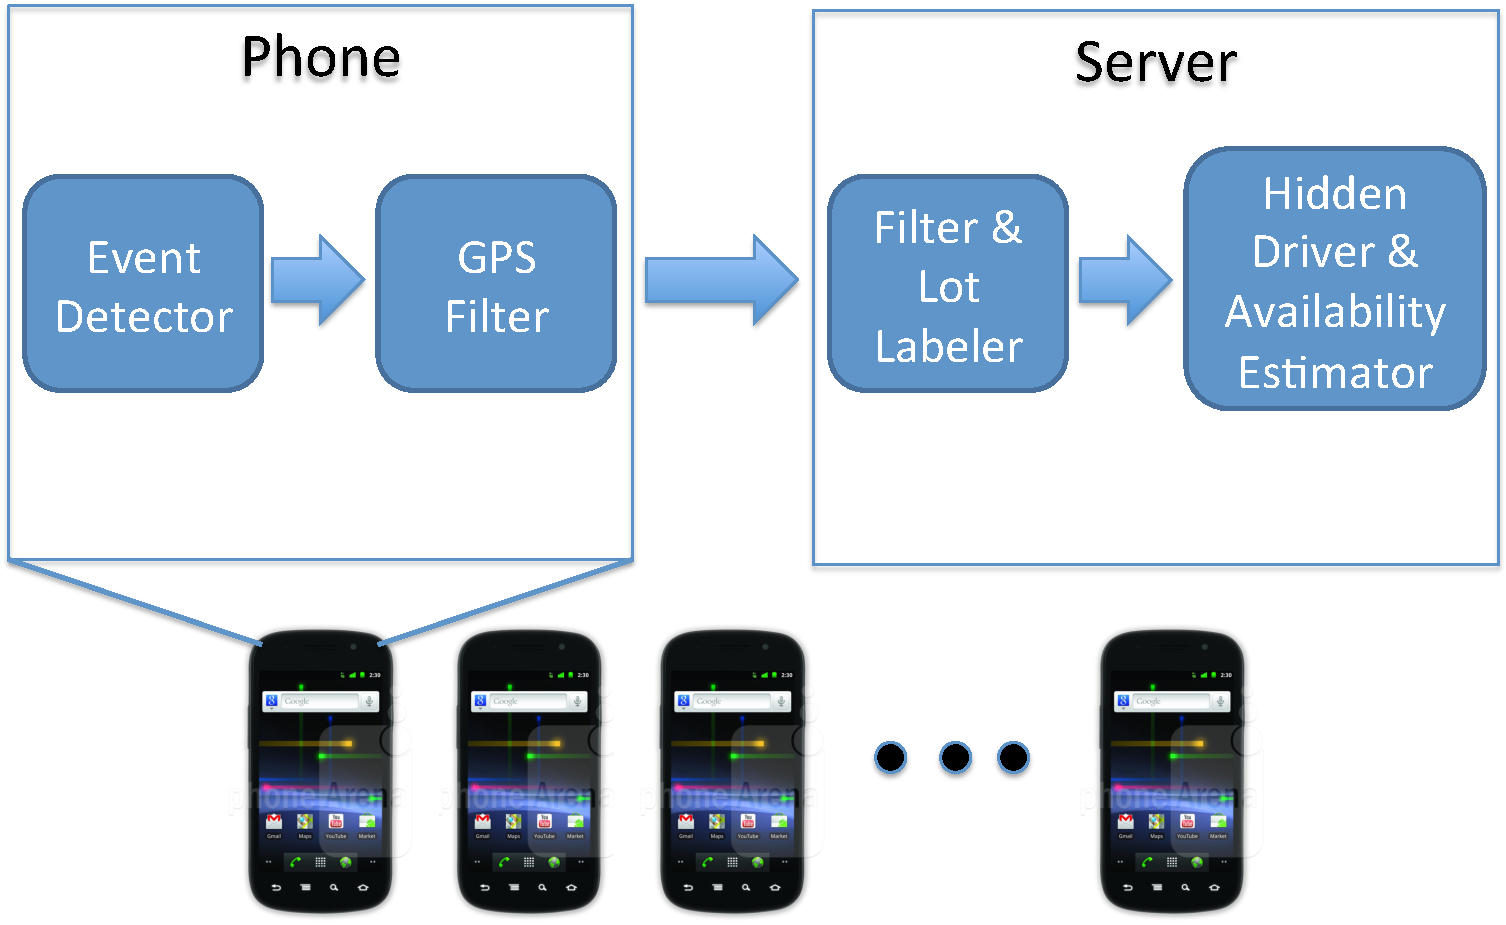
\includegraphics[width=\columnwidth]{./figures/blockdiagram.pdf}

\caption{\textbf{The PocketParker architecture.} Events generated by an
activity detector running quietly on each smartphone are processed by a
central server and used to estimate parking lot availability.}

\label{fig-arch}
\end{figure}
